\documentclass[11pt,a4paper]{article}

% Packages
\usepackage[utf8]{inputenc}
\usepackage[T1]{fontenc}
\usepackage{times}
\usepackage{graphicx}
\usepackage{booktabs}
\usepackage{hyperref}
\usepackage{geometry}
\usepackage{enumitem}
\usepackage{float}
\usepackage{tikz}
\usepackage{subcaption}
\usetikzlibrary{shapes.geometric, arrows.meta, positioning, fit, backgrounds}

% Page geometry
\geometry{margin=2.5cm}

% Hyperref settings
\hypersetup{
    colorlinks=true,
    linkcolor=blue!60!black,
    citecolor=blue!60!black,
    urlcolor=blue!60!black
}

% Graphics path
\graphicspath{{figures/}}

% Title
\title{\textbf{AI Academic Navigator: A Case Study of GPT-4 Powered Student Assessment in Higher Education}}

\author{
    Jan Saro\\
    Faculty of Economics and Management\\
    Czech University of Life Sciences Prague\\
    \texttt{saroj@pef.czu.cz}
}

\date{January 2026}

\begin{document}

\maketitle

\section*{Abstract}
This case study presents the AI Academic Navigator, a web-based platform leveraging GPT-4 for comprehensive cognitive assessment and personalized learning recommendations in higher education. Traditional psychometric assessments suffer from delayed feedback, generic interpretation, and low student engagement. Our platform addresses these limitations by integrating seven validated psychological instruments---including the Stroop Test, Mental Rotation Test, Grit Scale, and RIASEC career inventory---within an AI-guided interface that provides immediate, personalized synthesis. Deployed at the Czech University of Life Sciences Prague with 120 first-year business students, the system achieved 74\% completion rate, significantly exceeding typical paper-based assessments. The privacy-first architecture stores all assessment data client-side, addressing GDPR requirements while enabling rich AI-powered personalization. We present the system architecture, user experience flow, implementation results, and key lessons learned for educators considering AI integration in student assessment.

\vspace{0.5em}
\noindent\textbf{Keywords:} artificial intelligence, cognitive assessment, personalized learning, GPT-4, higher education, learning analytics

\vspace{0.5em}
\noindent\textbf{Track:} Teaching \& Learning --- AI-enhanced pedagogy and assessment

\section{Context and Motivation}

Higher education institutions increasingly recognize the importance of understanding individual student differences for effective teaching. Traditional psychometric assessments, while scientifically validated, present significant practical limitations in classroom settings. Students typically receive delayed feedback---often days or weeks after completion---reducing the immediate relevance of results. Interpretations tend to be generic, failing to connect findings to students' specific academic contexts or career aspirations. When multiple instruments are administered, results remain fragmented across separate reports, leaving students unable to see meaningful patterns across their cognitive profile.

Perhaps most critically, completion rates for traditional paper-based assessments rarely exceed 50\% in voluntary settings, as students perceive them as bureaucratic exercises disconnected from their learning experience. The emergence of large language models, particularly GPT-4, presented an opportunity to address these limitations---not by replacing validated instruments, but by enhancing interpretation, integration, and personalization in ways previously impossible at scale.

\section{System Architecture}

The AI Academic Navigator follows a privacy-first, client-centric architecture (Figure~\ref{fig:architecture}). Assessment data remains on the student's device, with only anonymized prompts sent to GPT-4 for synthesis.

\begin{figure}[H]
\centering
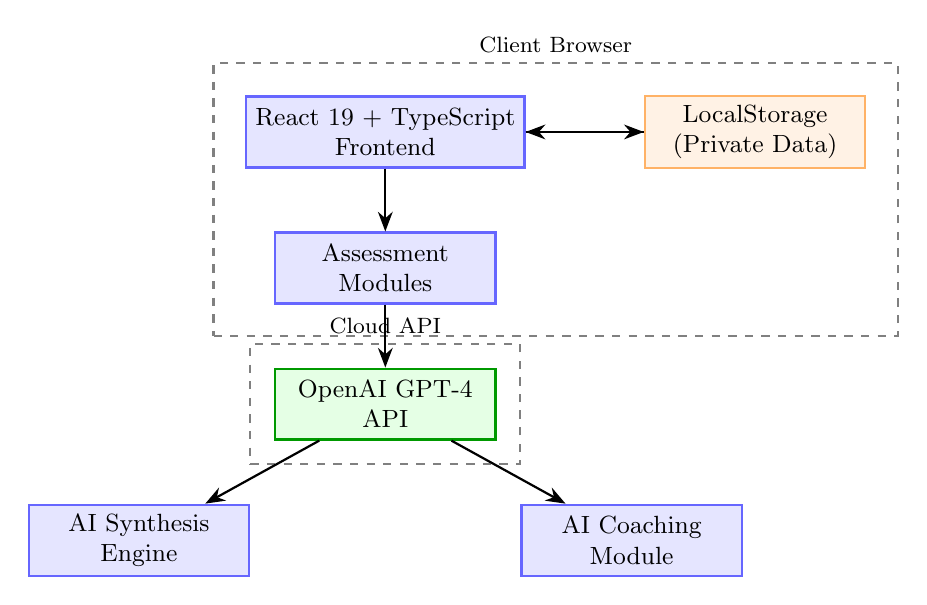
\begin{tikzpicture}[
    node distance=1.2cm,
    box/.style={rectangle, draw=blue!60, fill=blue!10, thick, minimum width=2.8cm, minimum height=0.9cm, align=center, font=\small},
    aibox/.style={rectangle, draw=green!60!black, fill=green!10, thick, minimum width=2.8cm, minimum height=0.9cm, align=center, font=\small},
    databox/.style={rectangle, draw=orange!60, fill=orange!10, thick, minimum width=2.8cm, minimum height=0.9cm, align=center, font=\small},
    arrow/.style={-{Stealth[length=2.5mm]}, thick}
]

% Client Layer
\node[box] (react) {React 19 + TypeScript\\Frontend};
\node[databox, right=1.5cm of react] (local) {LocalStorage\\(Private Data)};
\node[box, below=0.8cm of react] (modules) {Assessment\\Modules};

% AI Layer
\node[aibox, below=0.8cm of modules] (api) {OpenAI GPT-4\\API};

% Output Layer
\node[box, below left=0.8cm and 0.3cm of api] (synthesis) {AI Synthesis\\Engine};
\node[box, below right=0.8cm and 0.3cm of api] (coach) {AI Coaching\\Module};

% Arrows
\draw[arrow] (react) -- (local);
\draw[arrow] (local) -- (react);
\draw[arrow] (react) -- (modules);
\draw[arrow] (modules) -- (api);
\draw[arrow] (api) -- (synthesis);
\draw[arrow] (api) -- (coach);

% Background boxes
\begin{scope}[on background layer]
    \node[draw=gray, dashed, thick, fit=(react)(local)(modules), inner sep=0.4cm, label={[font=\footnotesize]above:Client Browser}] {};
    \node[draw=gray, dashed, thick, fit=(api), inner sep=0.3cm, label={[font=\footnotesize]above:Cloud API}] {};
\end{scope}

\end{tikzpicture}
\caption{System Architecture: Privacy-First Design}
\label{fig:architecture}
\end{figure}

\textbf{Technology Stack:}
\begin{itemize}[noitemsep]
    \item \textbf{Frontend:} React 19, TypeScript, Tailwind CSS
    \item \textbf{AI Integration:} OpenAI GPT-4 API
    \item \textbf{Data:} Client-side localStorage (GDPR compliant)
    \item \textbf{Languages:} Bilingual Czech/English interface
\end{itemize}

\section{User Experience Flow}

Students progress through a structured journey from assessment to personalized recommendations (Figure~\ref{fig:flow}).

\begin{figure}[H]
\centering
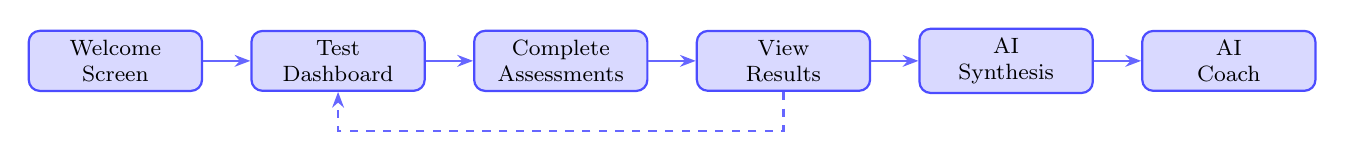
\begin{tikzpicture}[
    node distance=0.8cm,
    flowbox/.style={rectangle, rounded corners, draw=blue!70, fill=blue!15, thick, minimum width=2.2cm, minimum height=0.7cm, align=center, font=\footnotesize},
    arrow/.style={-{Stealth[length=2mm]}, thick, blue!60}
]

\node[flowbox] (welcome) {Welcome\\Screen};
\node[flowbox, right=0.6cm of welcome] (dashboard) {Test\\Dashboard};
\node[flowbox, right=0.6cm of dashboard] (assess) {Complete\\Assessments};
\node[flowbox, right=0.6cm of assess] (results) {View\\Results};
\node[flowbox, right=0.6cm of results] (synthesis) {AI\\Synthesis};
\node[flowbox, right=0.6cm of synthesis] (coach) {AI\\Coach};

\draw[arrow] (welcome) -- (dashboard);
\draw[arrow] (dashboard) -- (assess);
\draw[arrow] (assess) -- (results);
\draw[arrow] (results) -- (synthesis);
\draw[arrow] (synthesis) -- (coach);

% Loop back
\draw[arrow, dashed] (results.south) -- ++(0,-0.5) -| (dashboard.south);

\end{tikzpicture}
\caption{User Flow: From Assessment to AI-Powered Insights}
\label{fig:flow}
\end{figure}

\section{Platform Interface}

\subsection{Assessment Dashboard}

The dashboard (Figure~\ref{fig:dashboard}) presents all available assessments as interactive cards. Students can complete tests in any order, with visual progress indicators showing completion status.

\begin{figure}[H]
\centering
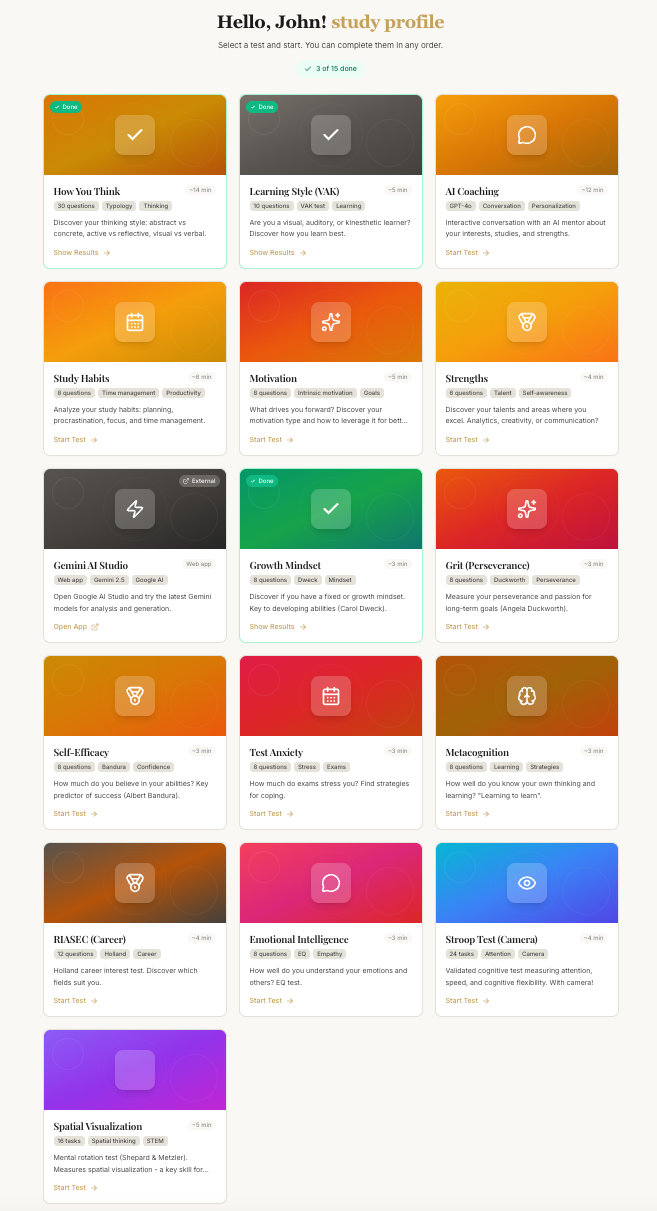
\includegraphics[width=0.85\textwidth]{dashboard.png}
\caption{Assessment Dashboard: Gallery-style interface with 16 cognitive and metacognitive tests}
\label{fig:dashboard}
\end{figure}

\subsection{AI Conversational Interview}

Beyond structured assessments, students engage in a GPT-4 powered conversational interview (Figure~\ref{fig:interview}). The AI explores interests, study habits, and career aspirations through natural dialogue, generating a comprehensive ``Student Passport'' report.

\begin{figure}[H]
\centering
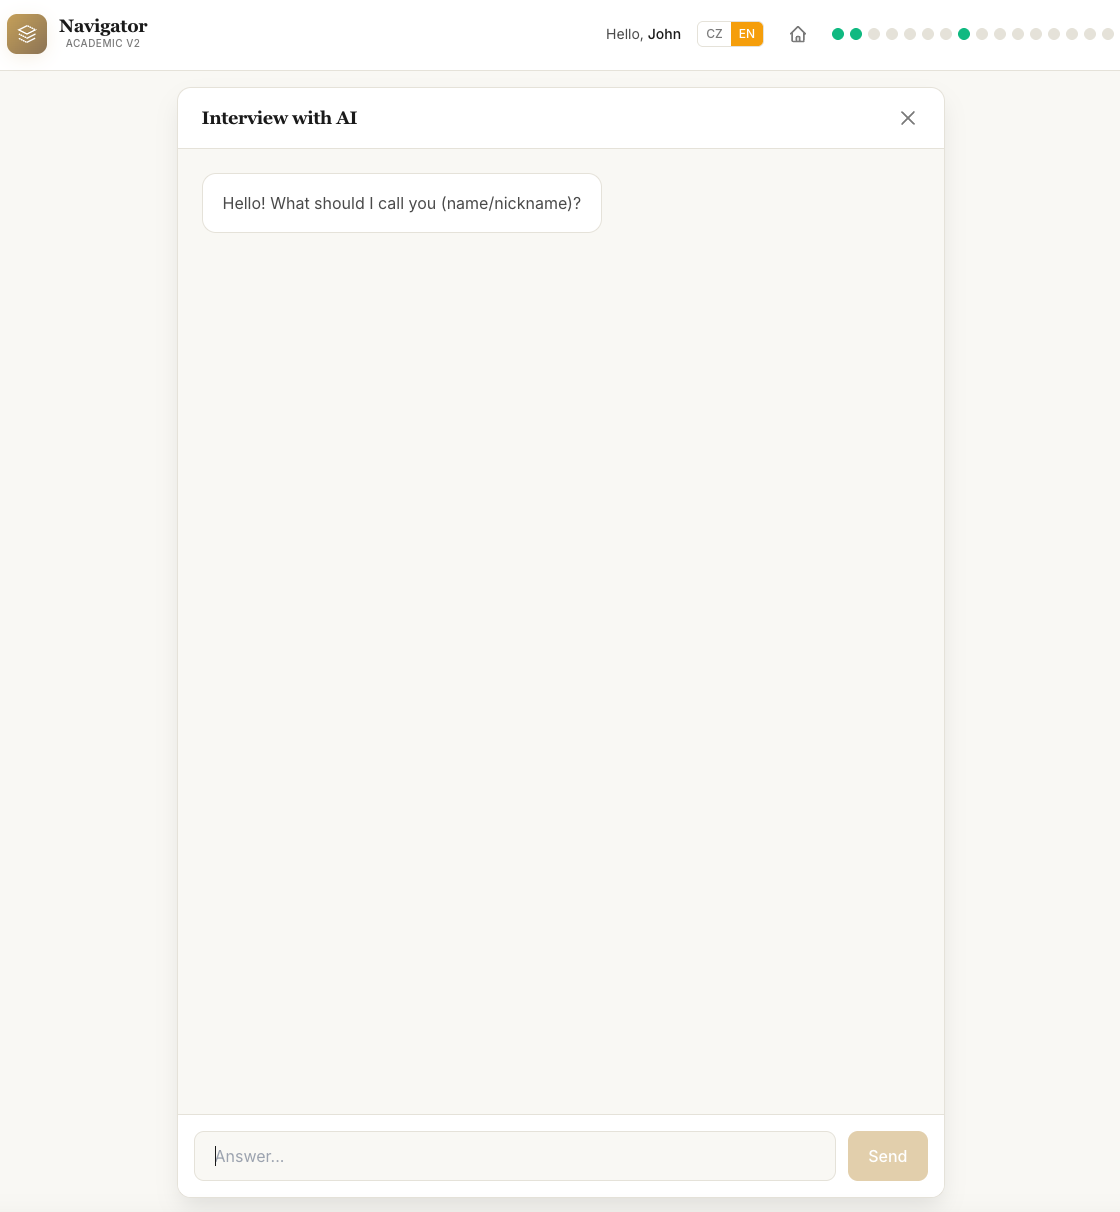
\includegraphics[width=0.85\textwidth]{ai-interview.png}
\caption{AI Interview: Natural conversation exploring student interests and goals}
\label{fig:interview}
\end{figure}

\subsection{AI Synthesis and Recommendations}

After completing assessments, GPT-4 synthesizes all results into a coherent learning profile (Figure~\ref{fig:synthesis}). The AI identifies patterns across instruments---for example, correlating visual learning preference with spatial ability scores and career interests.

\begin{figure}[H]
\centering
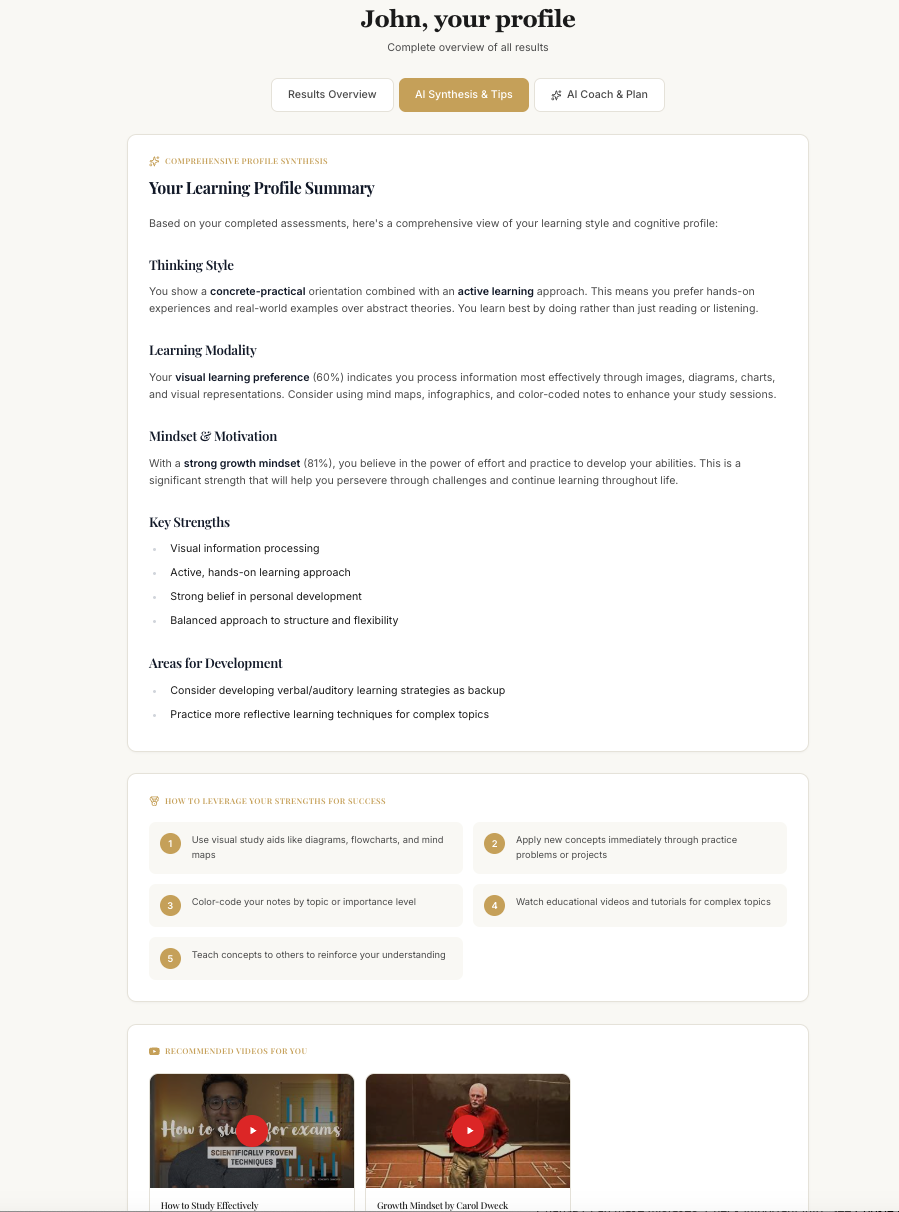
\includegraphics[width=0.85\textwidth]{ai-synthesis.png}
\caption{AI Synthesis: Integrated analysis with personalized study tips and video recommendations}
\label{fig:synthesis}
\end{figure}

\subsection{AI Coaching Module}

The coaching module (Figure~\ref{fig:coach}) transforms assessment data into actionable plans: weekly study schedules, habit trackers, and motivational guidance tailored to each student's cognitive profile.

\begin{figure}[H]
\centering
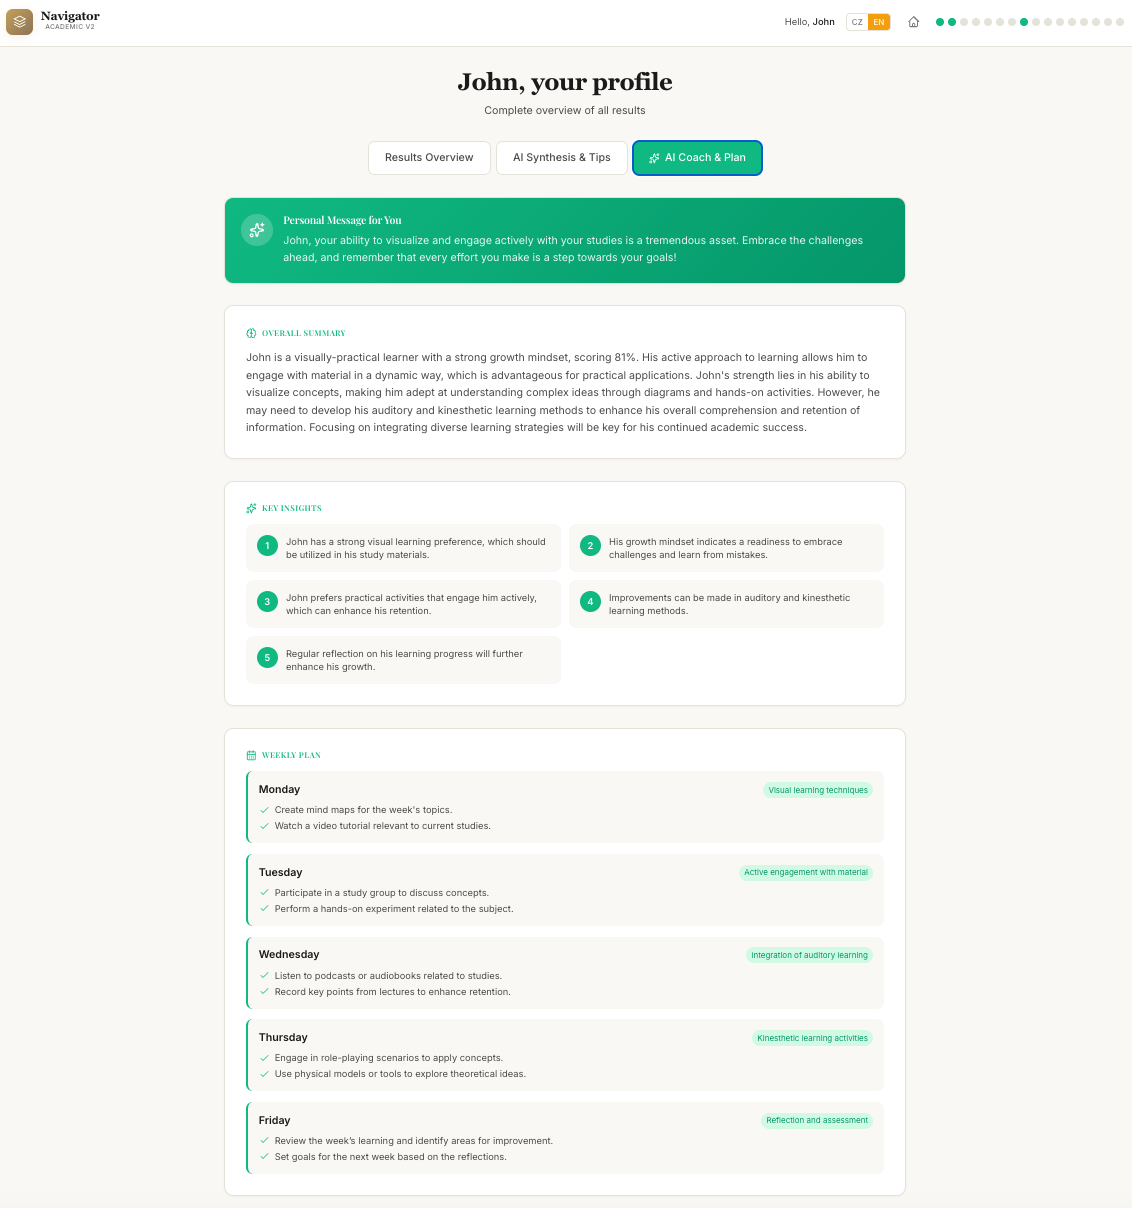
\includegraphics[width=0.85\textwidth]{ai-coach.png}
\caption{AI Coach: Personalized weekly plan and habit tracking based on assessment results}
\label{fig:coach}
\end{figure}

\section{Integrated Assessments}

The platform incorporates seven validated psychological instruments:

\begin{table}[H]
\centering
\small
\begin{tabular}{@{}lll@{}}
\toprule
\textbf{Module} & \textbf{Theoretical Basis} & \textbf{Measures} \\
\midrule
Stroop Test & Stroop (1935) & Selective attention, cognitive flexibility \\
Mental Rotation & Shepard \& Metzler (1971) & Spatial visualization ability \\
VAK Assessment & Fleming (1987) & Visual/Auditory/Kinesthetic preference \\
Grit Scale & Duckworth (2007) & Perseverance and passion \\
Growth Mindset & Dweck (2006) & Beliefs about intelligence malleability \\
RIASEC & Holland (1959) & Career interest typology \\
Emotional Intelligence & Goleman (1995) & Self and social awareness \\
\bottomrule
\end{tabular}
\caption{Validated Assessment Modules}
\end{table}

\section{Implementation Results}

The platform was piloted with 120 first-year business students at the Czech University of Life Sciences Prague during Fall 2025. Students accessed the platform during an introductory course on study skills, with participation voluntary but encouraged.

\textbf{Engagement Metrics:} Of 120 enrolled students, 89 (74\%) completed the full assessment battery---a completion rate significantly exceeding the 45--50\% typically observed with paper-based instruments at our institution. Analytics revealed that 34 students (38\% of completers) returned to the platform multiple times, primarily to re-read AI synthesis reports or explore the coaching module. Average session duration was 42 minutes, with students completing an average of 5.2 assessments per session.

\textbf{Personalization Quality:} Qualitative review of AI-generated syntheses demonstrated GPT-4's ability to integrate cross-instrument patterns meaningfully. For example, one student with strong visual learning preference (VAK), high spatial ability (Mental Rotation), and investigative career interest (RIASEC) received specific recommendations for data visualization coursework and research methodology---connections that would be difficult to derive from individual test reports alone. The AI coaching module generated 89 unique weekly study plans, each reflecting the student's specific cognitive profile and self-reported goals.

\textbf{Student Feedback:} Informal feedback indicated students particularly valued the immediate results, the conversational AI interview format, and the integration of multiple assessments into a coherent narrative. Several students reported sharing their AI synthesis with academic advisors during course selection consultations.

\textbf{Technical Performance:} AI synthesis generation averaged 3.2 seconds (SD=1.1s). The bilingual Czech/English interface served both domestic and international students effectively, with 23\% of completers using the English interface.

\section{Lessons Learned}

Our implementation experience yielded several insights relevant to educators considering similar AI integrations:

\begin{enumerate}[noitemsep]
    \item \textbf{AI augments, not replaces:} The most effective use of GPT-4 was enhancing validated instruments with personalized interpretation, not generating original assessments. Students trusted results because underlying instruments had established scientific validity.
    \item \textbf{Integration creates value:} Cross-assessment synthesis provided insights no single test could deliver. Connecting learning style preferences with career interests and cognitive abilities created actionable guidance that standalone reports cannot match.
    \item \textbf{Privacy enables trust:} Client-side data storage addressed GDPR concerns while maintaining full personalization capability. Students expressed comfort knowing their assessment data never left their devices.
    \item \textbf{Framing matters:} Students needed explicit guidance that AI recommendations complement, not replace, academic advising. We added disclaimers and encouraged students to discuss AI insights with human advisors.
    \item \textbf{Immediate feedback drives engagement:} The dramatic improvement in completion rates (74\% vs. typical 50\%) appears directly linked to immediate AI-generated feedback, transforming assessment from a passive data collection exercise into an interactive self-discovery experience.
\end{enumerate}

\section{Conclusion and Future Directions}

The AI Academic Navigator demonstrates practical integration of large language models into higher education assessment. By combining validated psychological instruments with GPT-4's analytical and synthesis capabilities, we provide personalized, actionable insights at scale that were previously available only through individual consultations with trained counselors.

Our pilot results suggest that AI-enhanced assessment addresses key limitations of traditional approaches: delayed feedback becomes immediate, generic interpretation becomes personalized, and fragmented results become integrated narratives. The 74\% completion rate indicates that students perceive genuine value in AI-mediated self-assessment.

Future development will focus on longitudinal tracking---connecting initial assessments with academic outcomes to validate AI recommendations---and expanding the instrument battery to include domain-specific assessments for different academic programs. The future of AI in education lies not in replacement but in augmentation: helping students understand themselves better and chart more effective learning paths.

\section*{Acknowledgments}
Supported by the Faculty of Economics and Management, Czech University of Life Sciences Prague.

\begin{thebibliography}{9}

\bibitem{duckworth2007}
Duckworth, A.L., et al. (2007).
Grit: Perseverance and passion for long-term goals.
\emph{J. of Personality and Social Psychology}, 92(6), 1087--1101.

\bibitem{dweck2006}
Dweck, C.S. (2006).
\emph{Mindset: The New Psychology of Success}. Random House.

\bibitem{fleming1987}
Fleming, N.D. (1987).
\emph{Teaching and Learning Styles: VARK Strategies}.

\bibitem{goleman1995}
Goleman, D. (1995).
\emph{Emotional Intelligence}. Bantam Books.

\bibitem{holland1959}
Holland, J.L. (1959).
A theory of vocational choice.
\emph{J. of Counseling Psychology}, 6(1), 35--45.

\bibitem{openai2023}
OpenAI (2023).
GPT-4 Technical Report. \emph{arXiv:2303.08774}.

\bibitem{shepard1971}
Shepard, R.N., \& Metzler, J. (1971).
Mental rotation of three-dimensional objects.
\emph{Science}, 171(3972), 701--703.

\bibitem{stroop1935}
Stroop, J.R. (1935).
Studies of interference in serial verbal reactions.
\emph{J. of Experimental Psychology}, 18(6), 643--662.

\end{thebibliography}

\end{document}
